%===================================================================================
% Chapter: Proposed Solution
%===================================================================================
\Chapter{Propuesta de Solución}\label{chapter:proposed_solution}
\vspace{-0.2in}
Esta investigación busca poder expresar un corpus anotado a través de una ontología definida, generando un grafo de conocimiento como resultado. Otro de los objetivos claros, es poder hacer esto mediante un algoritmo computacional, el cual debe ser, además, finito y determinista. 
%===================================================================================

\section{Analizador sintáctico}
Primeramente, es necesaria la creación de una herramienta capaz de fragmentar en objetos con significado computacional el contenido de los archivos de anotación escritos con el formato visto en la sección \ref{section:annotation_file_format}.

Dado que en el formato de archivo propuesto contiene una única relación anotada por línea y a su vez, las relaciones tienen su formato de escritura bien definido y sin ambigüedades, llevar a cabo la implementación de este analizador sintáctico es bastante sencillo. Esto puede hacerse a través de expresiones regulares, las cuales son ampliamente usadas y muchos de los lenguajes de programación modernos las incluyen como estructuras integradas.

\section{Modelo ontológico}
La ontología propuesta es de propósito general y basada en el modelo de anotación visto en la sección \ref{section:annotation_structure}. Esto posibilita la continuidad del proceso, partiendo desde documentos escritos en lenguaje natural, hasta la creación de una base de conocimiento a partir de ellos.

\subsection{Clases en la ontología}
La ontología se basa en tres clases fundamentales:

\begin{itemize}
	\item[•] Entidad simple: la más sencilla de las clases, no tiene ningún significado especial. En el modelo de la sección \ref{section:annotation_structure} representa un concepto sin haberle aplicado relaciones.
	\item[•] Entidad con atributo: está compuesta por una \textit{entidad simple} y uno o más atributos de los mencionados en la sección \ref{section:annotation_structure}. Puede verse como el resultado de haber aplicado todos los atributos pertenecientes a un mismo concepto.
	\item[•] Entidad compuesta: está compuesta por dos o más entidades, estas pueden ser de cualquier tipo. Puede verse como el resultado de aplicar las relaciones en el modelo de anotación explicado en la sección \ref{section:annotation_structure}.
\end{itemize}

Estas clases contienen, además, dos propiedades; una de ellas es la palabra o fragmento de texto en sí que representa la entidad y la otra es el tipo de concepto al que representan. Esta última propiedad se basa en los cuatro tipos de concepto existentes en el modelo de anotación explicado en la sección \ref{section:annotation_structure}, estos son: \textit{Concept}, \textit{Action}, \textit{Reference} y \textit{Predicate}.

\subsection{Relaciones en la ontología}
Los trece tipos de relación vistos en la sección \ref{section:relation_annotation} son relaciones válidas para este modelo. Estas, a su vez, pueden originarse y terminar en cualquiera de las tres posibles clases de la ontología propuesta.

Estas relaciones cobran el mismo significado semántico que en la sección \ref{section:annotation_structure}, estos son: {\it subject}, {\it target}, {\it domain}, {\it argument}, {\it is-a}, {\it part-of}, {\it same-as}, {\it has-property}, {\it causes}, {\it entails}, {\it in-time}, {\it in-place} o {\it in-context}.

En esta ocasión, los implicados en las relaciones son entidades de la ontología, y por ende, la palabra o fragmento de texto que estas representan. El proceso de creación de una base de conocimiento específica a partir de la definición de esta ontología es llevado a cabo de forma totalmente automática y no de la manera tradicional, con expertos en el dominio añadiendo relaciones entre clases una tras otra. A la interrogante de en qué orden se llevan a cabo estas relaciones y quiénes participan en ellas se le da respuesta en la próxima sección.

\section{Grafo de conocimiento}
Una vez que se haya analizado sintácticamente todo el corpus, se tendrá la información de las anotaciones en objetos computacionales y será más sencillo el trabajo con estos. En aras de evitar ambigüedades y concentrar el conocimiento para un mejor entendimiento de este y a la misma vez, poder facilitar la tarea de extraerlo de este grafo por un equipo de cómputo, el texto anotado es normalizado. Esto es llevado a cabo teniendo en cuenta las palabras que lo componen, y anotando en su lugar la palabra primitiva de esta. Por ejemplo, la palabra \guillemot{\texttt{sangramiento}} será anotada como \guillemot{\texttt{sangrar}} y la frase \guillemot{\texttt{glóbulos rojos}} como \guillemot{\texttt{glóbulo rojo}}.

Como se vio en la sección \ref{section:annotation_structure}, es necesario aclarar que hay que darle un orden a la creación de las instancias de las clases y las relaciones en este grafo, pues las propias anotaciones de texto y las relaciones tienen un orden implícito entre ellas. Por ejemplo, en la propia figura \ref{fig:annotation_example_composing_concepts}, se debe procesar primero el rol ejercido por \guillemot{\texttt{problemas}} y por \guillemot{\texttt{cumpla}} antes de poder procesar \guillemot{\texttt{impiden}}; de lo contrario, el conocimiento descrito por \guillemot{\texttt{impiden}} quedaría incompleto o mal representado.

\subsection{Orden topológico}
El orden establecido por el modelo de anotación visto en el capítulo \ref{chapter:annotation_model} es un orden topológico. Para ello se tiene en cuenta el siguiente orden:

\begin{enumerate}\label{enum:knowledge_graph_build_order}
	\vspace{-0.1in}
	\item Texto
	\vspace{-0.1in}
	\item Atributos
	\vspace{-0.1in}
	\item Relaciones de acción, predicado y contextualización
	\vspace{-0.1in}
	\item Relaciones taxonómicas y de causa e implicación
\end{enumerate}

Es válido aclarar que una vez divididas las relaciones en estos tres grupos, estas son asociadas nuevamente, esta vez teniendo en cuenta la parte izquierda de cada una de ellas (\texttt{Arg1} en el archivo de anotación). Se crea una instancia de clase por cada una de estas agrupaciones, una instancia creada en un nivel más avanzado, teniendo en cuenta el orden visto anteriormente, representa una mayor cantidad de información y al mismo tiempo, información más específica respecto a su instancia asociada en niveles anteriores.

En la figura \ref{fig:text_document1} puede verse un ejemplo de documento de texto, en este caso contiene una sola oración para que sea sencillo y entendible, pero en la práctica estos archivos contienen muchas más.

En la figura \ref{fig:annotated_document1} se ve el documento anotado asociado a este. Como puede apreciarse, se siguieron los convenios establecidos en la sección \ref{section:annotation_conventions}.

En la figura \ref{fig:knowledge_graph1.3} se puede ver cómo queda el grafo de conocimiento resultante de este corpus. Este contiene un solo documento en esta ocasión, pero en la práctica usualmente tiene muchos más.

La flecha que puede haber en algunas líneas del ejemplo significa que esta en el documento es muy larga para ser mostrada en una única línea en el ejemplo y se continuará escribiendo debajo.

En estos ejemplos, las palabras o frases no son normalizadas para un mejor entendimiento en lenguaje natural y además, porque hay varias formas, métodos y decisiones de cómo normalizar palabras o frases.
\begin{annexample}
[backgroundcolor=black!5]
{\textwidth}
{fig:text_document1}
{Ejemplo 1: documento \doublequote{\texttt{desmayo.txt}}}
{Ejemplo 1: documento \doublequote{\texttt{desmayo.txt}}.}
	El desmayo (o síncope) es una pérdida temporal de la {\scriptsize $\hookrightarrow$}\\
	conciencia.
\end{annexample}

\begin{annexample}
[backgroundcolor=cyan!13]
{\textwidth}
{fig:annotated_document1}
{Ejemplo 1: documento \doublequote{\texttt{desmayo.ann}}}
{Ejemplo 1: documento \doublequote{\texttt{desmayo.ann}}.}
	\# Sentence 1: El desmayo (o síncope) es una pérdida {\scriptsize $\hookrightarrow$}\\
	temporal de la conciencia.\\
	\# Keyphrases\\
	T1\space\space Concept 3 10\space\space\space\space desmayo\\
	T2\space\space Concept 14 21\space\space\space síncope\\
	T3\space\space Action 30 37\space\space\space\space pérdida\\
	T4\space\space Concept 38 46\space\space\space temporal\\
	T5\space\space Concept 53 63\space\space\space conciencia\\
	\# Relations\\
	R1\space\space is-a Arg1:T1 Arg2:T3\\
	R2\space\space in-context Arg1:T3 Arg2:T4\\
	R3\space\space target Arg1:T3 Arg2:T5\\
	\textasteriskcentered\space\space\space same-as T1 T2
\end{annexample}

Siguiendo el orden establecido \hyperref[enum:knowledge_graph_build_order]{anteriormente}, se puede ver en la figura \ref{fig:knowledge_graph1.1} el grafo de conocimiento resultante luego de realizado el punto $1$ es:

\begin{figure}[H]
	\begin{center}
		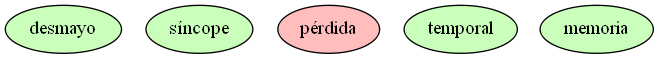
\includegraphics[width=4.5in]{graphics/knowledge_graph_example1_1.png}
		\caption[Ejemplo 1: grafo de conocimiento luego de realizado el punto 1]{Ejemplo 1: grafo de conocimiento luego de realizado el punto 1.}
		\label{fig:knowledge_graph1.1}
	\end{center}
\end{figure}

En el punto $2$ no hay nada que hacer en este corpus, pues no hay atributos, por tanto, el grafo de conocimiento quedará idéntico. Para el punto $3$ son usadas las relaciones \texttt{R2} y \texttt{R3}, resultando:
\begin{figure}[H]
	\begin{center}
		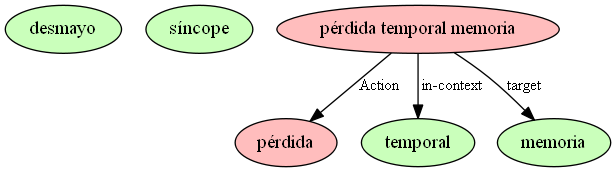
\includegraphics[width=4.7in]{graphics/knowledge_graph_example1_2.png}
		\caption[Ejemplo 1: grafo de conocimiento luego de realizado el punto 3]{Ejemplo 1: grafo de conocimiento luego de realizado el punto 3.}
		\label{fig:knowledge_graph1.2}
	\end{center}
\end{figure}

Para el punto $4$ son usadas las relaciones restantes: \texttt{R1} y \texttt{\textasteriskcentered}. Resultando:
\begin{figure}[H]
	\begin{center}
		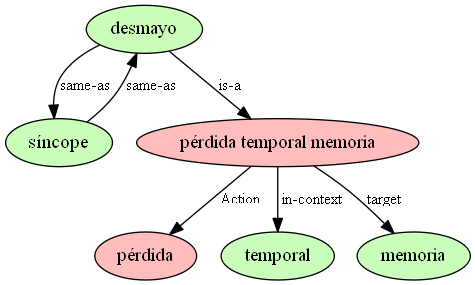
\includegraphics[width=3.6in]{graphics/knowledge_graph_example1_3.png}
		\caption[Ejemplo 1: grafo de conocimiento luego de realizado el punto 4]{Ejemplo 1: grafo de conocimiento luego de realizado el punto 4.}
		\label{fig:knowledge_graph1.3}
	\end{center}
\end{figure}

El ejemplo anterior es sencillo y muestra un documento con una única oración también sencilla. Ahora se muestra un ejemplo de un corpus que igualmente contiene un solo documento compuesto por una oración, pero esta vez, una oración más compleja y que abarca todos los grupos de relaciones que hay en el modelo de anotación.

La figura \ref{fig:text_document2} muestra el documento de texto, en la \ref{fig:annotated_document2} se aprecia su respectivo archivo anotado y en la \ref{fig:knowledge_graph2.4} el resultado final del grafo de conocimiento.

\begin{annexample}
[backgroundcolor=black!5]
{\textwidth}
{fig:text_document2}
{Ejemplo 2: documento \doublequote{\texttt{higiene.txt}}}
{Ejemplo 2: documento \doublequote{\texttt{higiene.txt}}.}
	Las buenas prácticas de higiene, incluyendo lavarse las {\scriptsize $\hookrightarrow$}\\
	manos correctamente, pueden evitar infecciones.
\end{annexample}

\begin{annexample}
[backgroundcolor=cyan!13]
{\textwidth}
{fig:annotated_document2}
{Ejemplo 2: documento \doublequote{\texttt{higiene.ann}}}
{Ejemplo 2: documento \doublequote{\texttt{higiene.ann}}.}
	\# Sentence 1: Las buenas prácticas de higiene, incluyendo {\scriptsize $\hookrightarrow$}\\
	lavarse las manos correctamente, pueden evitar infecciones.\\
	\# Keyphrases\\
	T1\space\space Concept 4 10\space\space\space\space buenas\\
	T2\space\space Predicate 11 20 prácticas\\
	T3\space\space Concept 24 31\space\space\space higiene\\
	T4\space\space Action 44 51\space\space\space\space lavarse\\
	T5\space\space Concept 56 61\space\space\space manos\\
	T6\space\space Concept 62 75\space\space\space correctamente\\
	T7\space\space Action 84 90\space\space\space\space evitar\\
	T8\space\space Concept 91 102\space\space infecciones\\
	\# Relations\\
	R1\space\space in-context Arg1:T2 Arg2:T1\\
	R2\space\space domain Arg1:T2 Arg2:T3\\
	R3\space\space causes Arg1:T2 Arg2:T7\\
	R4\space\space is-a Arg1:T4 Arg2:T2\\
	R5\space\space target Arg1:T4 Arg2:T5\\
	R6\space\space in-context Arg1:T4 Arg2:T6\\
	R7\space\space target Arg1:T7 Arg2:T8\\
	\# Attributes\\
	A1\space\space Uncertain T7
\end{annexample}

Una vez más, siguiendo el orden establecido \hyperref[enum:knowledge_graph_build_order]{anteriormente}, se puede ver en la figura \ref{fig:knowledge_graph2.1} el grafo de conocimiento resultante luego de realizado el punto $1$.

\begin{figure}[H]
	\begin{center}
		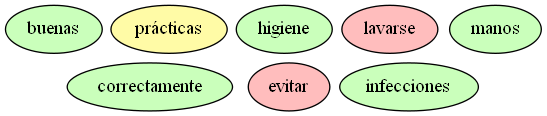
\includegraphics[width=4.2in]{graphics/knowledge_graph_example2_1.png}
		\caption[Ejemplo 2: grafo de conocimiento luego de realizado el punto 1]{Ejemplo 2: grafo de conocimiento luego de realizado el punto 1.}
		\label{fig:knowledge_graph2.1}
	\end{center}
\end{figure}

Dándole solución al punto $2$, el grafo quedaría así:
\begin{figure}[H]
	\begin{center}
		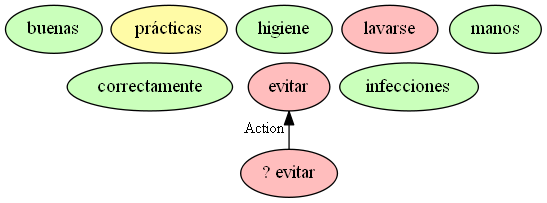
\includegraphics[width=4.2in]{graphics/knowledge_graph_example2_2.png}
		\caption[Ejemplo 2: grafo de conocimiento luego de realizado el punto 2]{Ejemplo 2: grafo de conocimiento luego de realizado el punto 2.}
		\label{fig:knowledge_graph2.2}
	\end{center}
\end{figure}

Una vez completado el punto $3$, este es el resultado:
\begin{figure}[H]
	\begin{center}
		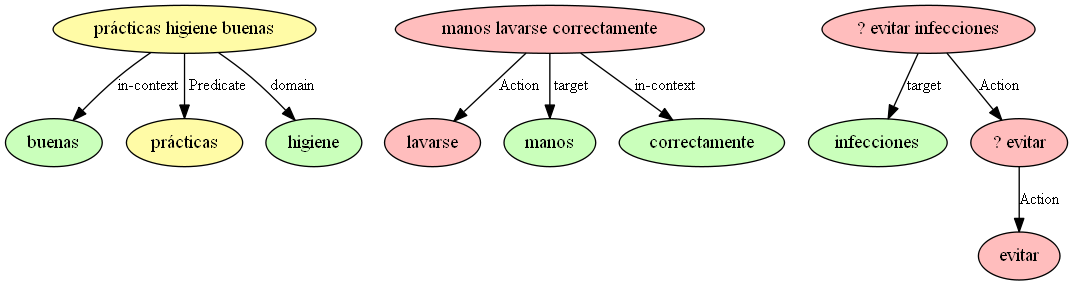
\includegraphics[width=\textwidth]{graphics/knowledge_graph_example2_3.png}
		\caption[Ejemplo 2: grafo de conocimiento luego de realizado el punto 3]{Ejemplo 2: grafo de conocimiento luego de realizado el punto 3.}
		\label{fig:knowledge_graph2.3}
	\end{center}
\end{figure}

Finalmente, al llevar a cabo el punto $4$, este sería el resultado:
\begin{figure}[H]
	\begin{center}
		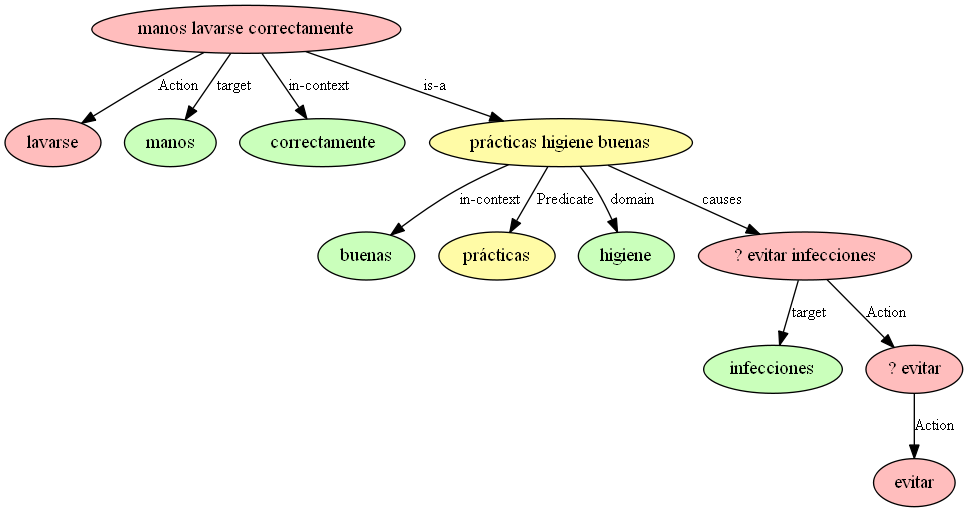
\includegraphics[width=\textwidth]{graphics/knowledge_graph_example2_4.png}
		\caption[Ejemplo 2: grafo de conocimiento luego de realizado el punto 4]{Ejemplo 2: grafo de conocimiento luego de realizado el punto 4.}
		\label{fig:knowledge_graph2.4}
	\end{center}
\end{figure}

Como pudo apreciarse en el ejemplo anterior, se optó por mostrar los atributos en el grafo a través de caracteres en vez de la palabra en sí. Son usados los siguientes caracteres:
\begin{itemize}
	\item[$\lnot$] negación
	\item[?] incertidumbre
	\item[$\downarrow$] disminución
	\item[$\uparrow$] énfasis
\end{itemize}

\subsection{Creación de instancias de clases}\label{section:ontology_construction}
Para llevar a cabo el punto $1$ en el orden previamente expuesto, se crea una \textit{entidad simple} por cada concepto existente en el documento de anotación. Esto sienta las bases para la posterior realización y correctitud del algoritmo expuesto en la sección anterior.

Para cumplimentar lo propuesto en el punto $2$, cumplen un papel protagónico las entidades de los conceptos que tienen atributos asociados. En este punto, todas estas son del tipo \textit{entidad simple} y cada una de ellas se une con todos sus respectivos atributos, formando una \textit{entidad con atributo}.

En el paso $3$ tienen lugar algunas de las relaciones. Cada una de ellas conforma una \textit{entidad compuesta}. Esta nueva instancia se relaciona con los conceptos de las partes derecha de dichas relaciones, ahora devenidos en alguno de los tres tipos de clases de esta ontología, a través del tipo de relación. A la vez que se relaciona con la parte izquierda de estas por medio del tipo de entidad que sean.

El paso $4$ no crea instancias nuevas, solo establece la relación entre dos instancias creadas previamente en el grafo, aportando así conocimiento al mismo.

\section{Resolución de correferencias}
La resolución de correferencias es la tarea de encontrar todas las expresiones que refieren a la misma entidad en un texto. Es un paso importante para muchos algoritmos de procesamiento de lenguaje natural y por tanto, lo es también para esta investigación.

Ejemplificando, es el problema de darse cuenta que en el fragmento de texto \doublequote{\textit{\dots\space si una ampolla es grande, dolorosa o parece que se reventará por sí sola, usted puede drenar el líquido. Esto debería reducir su dolor\dots}} la palabra \guillemot{\texttt{Esto}} hace referencia a \guillemot{\texttt{drenar el líquido}}.

En el marco del ámbito social y mundial en que fue hecha esta investigación y por motivos principalmente de recursos, no se pudo dar resultados concretos en esta tarea. Convirtiéndose así en un objetivo que con el paso del tiempo pasó de estar plenamente involucrado con este estudio a ser una recomendación para el futuro. De esta manera se dejan abiertas las puertas para la continuación y mejora de lo que aquí se presenta.